\chapter{\IfLanguageName{dutch}{Stand van zaken}{State of the art}}
\label{ch:stand-van-zaken}

% Tip: Begin elk hoofdstuk met een paragraaf inleiding die beschrijft hoe
% dit hoofdstuk past binnen het geheel van de bachelorproef. Geef in het
% bijzonder aan wat de link is met het vorige en volgende hoofdstuk.

% Pas na deze inleidende paragraaf komt de eerste sectiehoofding.
In deze stand van zaken worden de gebruikte technologieën stapsgewijs besproken om het nodige inzicht te creëren in het onderwerp chaos engineering. Eerst zal uitgelegd worden wat virtualisatie is en welke voordelen dit met zich meebrengt.
Vervolgens wordt toegelicht hoe softwareontwikkeling geëvolueerd is van een monolitische naar een microservices architectuur en hoe containerisatie hier een rol in speelt. Nadien zal uitleg gegeven worden over wat de containerorkestratie Kubernetes is, hoe het er voor zorgt dat applicaties dynamisch kunnen schalen en hoe er gemikt wordt naar een zo hoog mogelijke uptime ervan. Tot slot wordt besproken wat chaos engineering inhoudt en wat de link is met containerorkestratie.   

\section{Virtualisatie}

Virtualisatie maakt het mogelijk om op een fysieke computer meerdere virtuele machines uit te voeren, elk met zijn eigen besturingssysteem, geheugen, processorkernen en opslagcapaciteit.

Het essentiële onderdeel om de virtuele machines te binden aan de hardware van de fysieke host, en wat de dynamische toewijzing van resources zoals geheugen en CPU mogelijk maakt, is een softwarelaag die men de hypervisor noemt. 

\subsection{Voordelen van een hypervisor}

Het gebruik van een hypervisor om virtuele machines op een host aan te maken heeft enkele voordelen \autocite{Yfantis2020} :
\begin{itemize}
    \item Snelheid: virtuele machines opzetten verloopt snel in vergelijking met de tijd benodigd om een fysieke server op te zetten.
    \item (Kost)efficiëntie: men maakt optimaal gebruik van de beschikbare resources op het hostsysteem door deze dynamisch te verdelen over meerdere virtuele machines.   
    \item Overdraagbaarheid: virtuele machines worden bewaard als bestanden op de host en zijn makkelijk overdraagbaar naar andere systemen.
\end{itemize}

\subsection{Types hypervisors}

Er bestaan twee hypervisor types:
\begin{itemize}
    \item Type 1: bare-metal / native
    \item Type 2: hosted
\end{itemize}

Een bare-metal of native type 1 hypervisor is virtualisatiesoftware die rechtstreeks geïmplementeerd is op de hardware van een host en zich gedraagt zoals een lichtgewicht besturingssysteem. Het voordeel bij dit type hypervisor is dat geen volwaardig besturingssysteem geïnstalleerd wordt en dat het hiermee gevrijwaard blijft van de kwetsbaarheden die dit met zich meebrengt. Voorbeelden van type 1 hypervisors zijn VMware ESXi, Microsoft Hyper-V, Citrix Xen ... 

Een hosted type 2 hypervisor is software die bovenop het bestaande besturingssysteem op een host aanwezig is. Het nadeel bij een type 2 hypervisor is de verhoogde latentie doordat de communicatie tussen hardware en hypervisor eerst nog het besturingsssysteem moet passeren. Bekende voorbeelden hiervan zijn de softwarepakketten VirtualBox of VMware. 

\begin{figure}[h]
    \centering
    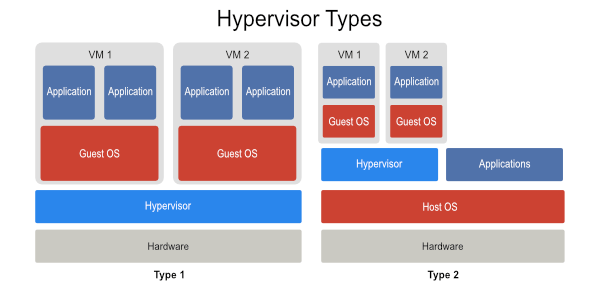
\includegraphics[scale=.6]{img/Hypervisor-Types.png}
    \caption{hypervisor types \autocite{Vembu2019}}
    \label{hypervisors}
\end{figure}

\section{Automatisatietools}
\subsection{Vagrant}

Vagrant is open-source software ontworpen door HashiCorp met als doel virtuele omgevingen op te zetten en te beheren. \autocite{Vagrant2022} Met behulp van een Vagrantfile, een configuratiebestand waarin specificaties van de omgeving gedefineerd zijn, kan men via het {\bf vagrant up} commando op een geautomatiseerde manier één of meerdere virtuele machines creëeren. 

De software VirtualBox dient hierbij alreeds op het systeem aanwezig te zijn, aangezien Vagrant standaard de virtuele machines achterliggend via deze hypervisor type 2 zal creëeren. \autocite{Vagrant2022a}

\subsection{Ansible}

Ansible is open-source configuratiemanagementsoftware ontworpen door RedHat. Het doel van Ansible is om repetitieve en manuele taken te automatiseren via verschillende scripts die gebundeld worden in een Ansible playbook. \autocite{RedHatAnsible2022} 

\section{Evolutie in softwarerachitectuur}

Klassieke softwareontwikkeling leverde applicaties op die gebaseerd waren op een monolitische architectuur. Hierin was alle code aanwezig van de applicatie, zowel front- als backend. 
Dit bracht verschillende voordelen met zich mee waaronder:
\begin{itemize}
    \item makkelijk qua ontwikkeling omdat IDEs/tools gefocust waren op het bouwen van 1 applicatie.
    \item vlotter om te testen gezien de code zich allemaal in 1 applicatie bevindt. 
    \item simpel om uit te rollen in productie omdat men de verpakte applicatie slechts moest kopiëren op een server. 
    \item schalen van de applicatie eenvoudig door meerdere kopieën uit te voeren achter een load balancer.
\end{itemize} 

Verschillende nadelen van deze manier van softwarontwikkeling kwamen echter aan het licht wanneer succesvolle applicaties met de tijd begonnen te groeien. Wanneer ontwikkelaars nieuwe functionaliteit wouden toevoegen werd steeds meer code toegevoegd, waardoor de complexiteit van de applicatie steeds verhoogde. Het resultaat hiervan was dat bugs oplossen en features toevoegen steeds moeizamer verliep. Elke keer een functionaliteit veranderde aan de applicatie moest de hele applicatie opnieuw uitgerold worden, wat voor continuous deployment een enorm obstakel is.
De betrouwbaarheid van een monolitische applicatie is ook een minpunt aangezien een bug ervoor kan zorgen dat de beschikbaarheid van de volledige applicatie in het gedrang komt. \autocite{Richardson2015}

Om deze problemen met monolitische applicaties aan te pakken gebruikten grote bedrijven zoals Amazon, eBay, en Netflix een nieuwe softwareontwikkeling op basis van een microservices architectuur. Het idee achter deze nieuwe manier van softwareontwikkelling is om de applicatie op te splitsen in verschillende kleine geconnecteerde services die elk een set van features of specifieke functionaliteit bevatten.

\begin{figure}[h]
    \centering
    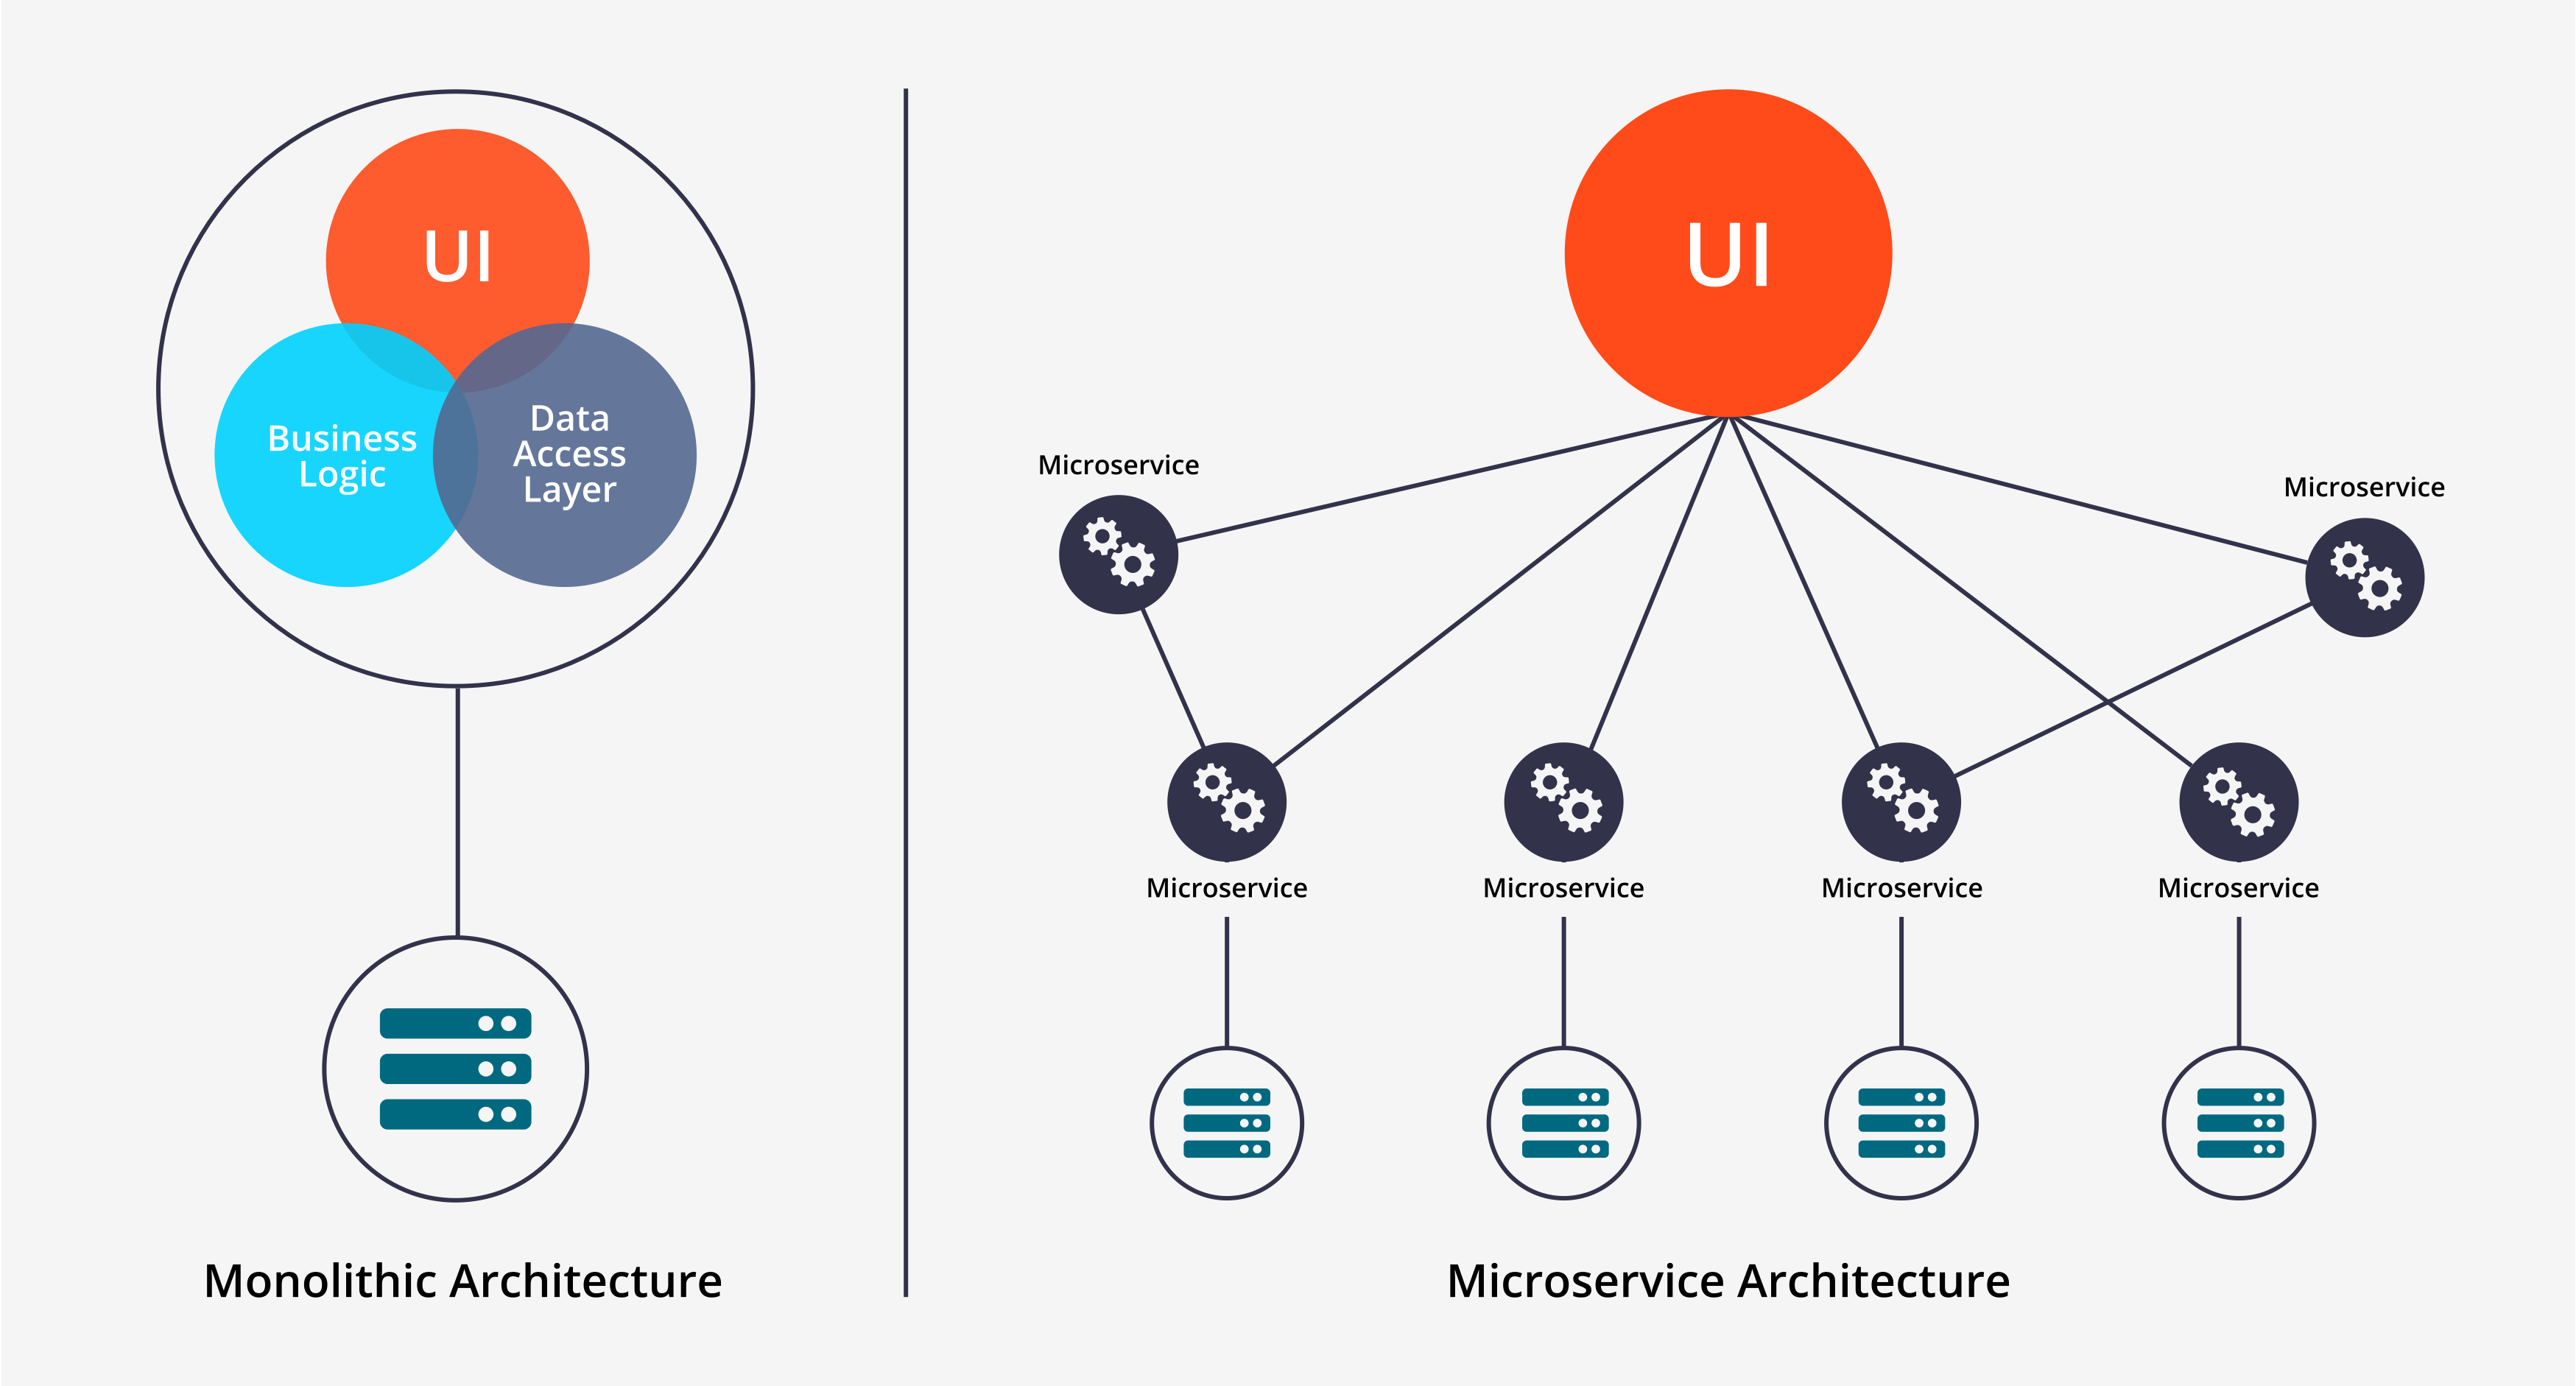
\includegraphics[scale=.1]{img/monolithic_vs_microservices.png}
    \caption{evoloutie in softwarearchitectuur \autocite{Sanjaya2020}}
    \label{softwarearchitectuur}
\end{figure}

\section{Containerisatie}

Applicaties gebouwd via een microservices architectuur brengen services onder in containers. Een container op zich bevat geen besturingssysteem maar verpakt en isoleert de code van één applicatie inclusief de gerelateerde configuratiebestanden en afhankelijkheden die deze nodig heeft. Het voordeel van containers is dat ze snel opgestart kunnen worden doordat ze weinig resources vereisen, en makkelijk overdraagbaar zijn naar verschillende omgevingen. Meerdere containers kunnen actief zijn op een systeem en maken ook allemaal gebruik van hetzelfde besturingssysteem. \autocite{Singh2020}

Ondanks dat containers net zoals virtuele machines een vorm van virtualisatie zijn, is er toch een belangrijk onderscheid te maken. Containers zijn namelijk een vorm van besturingssysteemvirtualisatie, dit tegenover virtuele machines die aan hardwarevirtualisatie doen.
Hierdoor verbruiken containers dus minder resources ten opzichte van virtuele machines. \autocite{Holt2018}

Containers en virtuele machines kunnen gecombineerd worden om virtuele omgevingen te maken waarin software ontwikkeld en getest kan worden. Containers blijven wel afhankelijk van het besturingssysteem. Men kan geen Windows containers in een Linux omgeving opstarten of omgekeerd. Om de interactie met het besturingssysteem op de host mogelijk te maken is een container runtime op het systeem nodig zoals Docker Engine, CRI-O, LXC ...

\subsection{Docker}

De oorsprong van containers kan herleid worden naar 1979 toen men voor het eerst een proces kon isoleren via de system call chroot in Unix V7. Pas vanaf 2000 kwamen bedrijven zoals Open Virtuzzo en Google met nieuwe ontwikkellingen zoals cgroups en LXC (Linux containers) die de concepten rond containerisatie meer vorm begonnen te geven. Het was pas echter toen Docker in 2013 op de markt kwam dat het gebruik van containers qua populariteit explodeerde. 
Docker maakte het onderscheid door een volledig ecosysteem aan te bieden voor container management.\autocite{Osnat2020} 

Door Docker Engine op het systeem te installeren kan men gecontaineriseerde applicaties op gelijk welke infrastructuur uitvoeren. Voordien kon men hinder ondervinden doordat afhankelijkheden van applicaties ervoor zorgden dat het uitvoeren ervan in een andere omgeving problemen kon geven. Dit probleem wordt vaak omschreven als de 'dependency hell'.

Met Docker bundelt een ontwikkelaar een applicatie en zijn afhankelijkheden in een container die overal uitvoerbaar is. Om een applicatie in een container te plaatsen is een Dockerfile nodig. 
Dit bestand plaatst men bij de applicatie en is in essentie een set instructies waarin de applicatiecode inclusief de benodigde afhankelijkheden gekopieerd worden naar de container en hoe de applicatie opgestart wordt. De Dockerfile zal vervolgens gebruikt worden om een image te maken, die opgeslagen wordt in een publieke repository zoals Docker Hub of een private repository.

Wanneer men de applicatie op een ander systeem wil opbouwen, waar Docker ook geïnstalleerd is, kan men via het docker run commando de image van de applicatie uit een repository halen en hiermee een container op het systeem lanceren die de applicatie bevat.  

\section{Containerorkestratie}

In een productieomgeving moet men ervoor zorgen dat applicaties continu beschikbaar blijven en deze fouttolerant zijn. Wanneer een container faalt, moet een andere container automatisch opgestart worden om dit op te vangen. Wanneer meer gebruik gemaakt wordt van een applicatie, moet deze automatisch kunnen schalen om deze extra vraag op te vangen. Om deze redenen en nog veel meer wordt containerorkestratie toegepast.

Containerorkestratie is het volledige proces rond het uitrollen, beheren en schalen van gecontaineriseerde applicaties. De bekendste speler in containerorchestratie is ongetwijfeld Kubernetes (K8s). Andere aanbieders in deze markt zijn o.a. Nomad, Docker Swarm, Amazon Elastic Kubernetes Service (EKS) ...
Bij het opzetten van de verschillende virtuele omgevingen die later in hoofdstuk 3 uitvoerig besproken worden werd enkel gebruik gemaakt van Kubernetes.

\subsection{Kubernetes} 

Ongeveer 1 jaar nadat de containerisatiesoftware Docker in 2013 op de markt verscheen, werd Kubernetes aan het grote publiek voorgesteld. Oorspronkelijk werd het ontwikkeld door Google, maar nu wordt het project onderhouden door de Cloud Native Computing Foundation (https://www.cncf.io/).

Kubernetes wordt op hun eigen website omschreven als een overdraagbaar, uit te breiden, open-source platform voor het beheer van gecontaineriseerde applicaties en services, dat zowel declaratieve als geautomatiseerde configuratie toelaat.

\subsection{Kubernetes architectuur}

Het grootste object in de Kubernetes architectuur noemt men een cluster. Hierin worden fysieke of virtuele machines als nodes gegroepeerd. Men kan afhankelijk van het aantal nodes twee types clusters onderscheiden:

\begin{itemize}
    \item een single-node cluster 
    \item een multi-node cluster 
\end{itemize} 

Wanneer men meerdere nodes in een cluster onderbrengt kan het onderscheid gemaakt worden tussen:

\begin{itemize}
    \item de control-plane node(s), in oudere versies nog de master node genoemd.
    \item de worker node(s)
\end{itemize} 

In een single-node cluster is de enige node zowel de control-plane als worker node.
Later in hoofdstuk \ref{ch:methodologie} zullen verschillende Kubernetes distributies gebruikt worden om een lokale cluster op te zetten. Hierbij zal zowel een single-node cluster via Minikube, alsook multi-node clusters via Kubeadm en Kubespray opgezet worden. Ook zal aangetoond worden hoe men via Google Kubernetes Engine (GKE) een cluster in Google Cloud kan opzetten.

De infrastructuur van een Kubernetes cluster bevat een aantal componenten die afhankelijk van het type node zullen geïnstalleerd worden. Op deze manier zijn de verantwoordelijkheden in een cluster duidelijk afgelijnd. De volgende componenten kan men in elke cluster terugvinden: 

\begin{itemize}
    \item {\bf API server}: de front-end voor de control-plane en laat interactie met een cluster toe. 
    \item {\bf etcd}: een key-value store die gebruikt wordt om clusterdata op te slaan. 
    \item {\bf scheduler}: verantwoordelijk voor de distributie van containers naar de nodes.
    \item {\bf controller}: verantwoordelijk voor het monitoren en reageren wanneer nodes/pods uitvallen en beslist als nieuwe nodes/pods gecreëerd moeten worden.
    \item {\bf container runtime}: de onderliggende software die het mogelijk maakt om containers uit te voeren bv. Docker. 
    \item {\bf kubelet}: een agent die op elke node actief is en verantwoordelijk is voor de correcte uitvoering van de containers.   
\end{itemize}

Elk infrastructuurcomponent hierboven opgesomd zal steeds ondergebracht worden in een pod, wat het kleinste Kubernetes object is. Meer over pods kan u later lezen in sectie \ref{sec:workloads}.
De API-server, etcd, scheduler en controller zijn de componenten die verantwoordelijk zijn voor het beheer van de cluster en zijn samen gebundeld in de control-plane node. Deze staat in voor het beheer van de worker nodes en de pods in de cluster.

Een worker node bevat de pods van een workload, of anders geformuleerd de containers van een applicatie. De kubelet en een kube-proxy zijn de enige infrastructuurcomponenten benodigd op een worker node. De kubelet is verantwoordelijk voor de communicatie met de control-plane node en zal deze eveneens informeren over de interne staat van de worker node. De kube-proxy staat in voor de netwerkcommunicatie. 

Een overzicht van de verschillende infrastructuurcomponenten en de onderverdeling over de verschillende nodes kan u zien in figuur \ref{k8s-architectuur}. 

\begin{figure}[h]
    \centering
    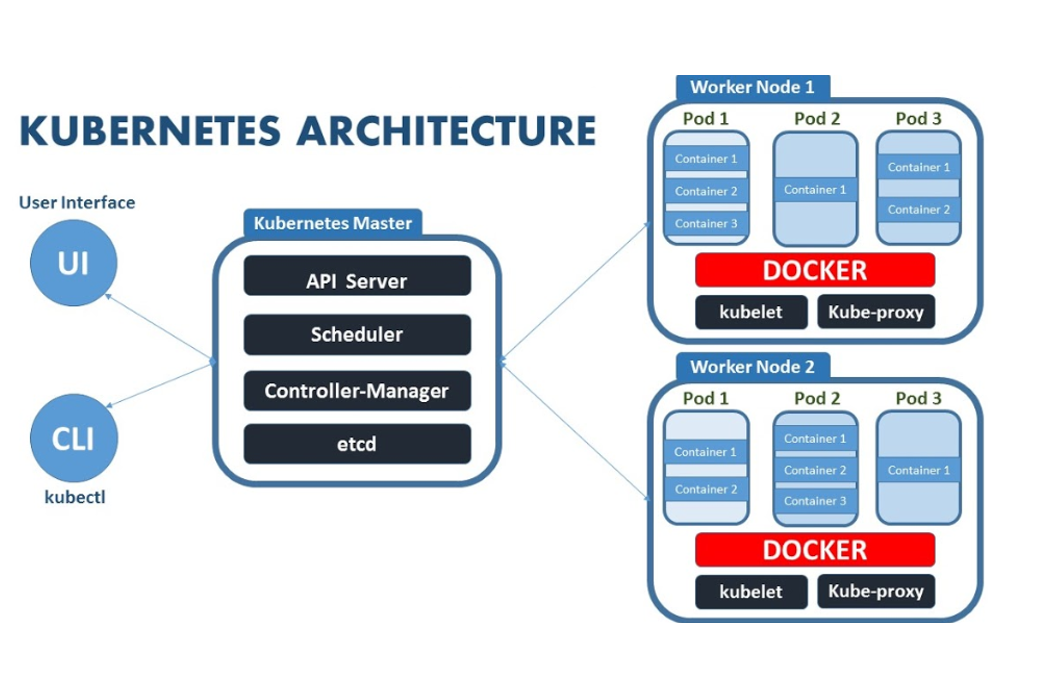
\includegraphics[scale=.7]{img/k8s-architecture.png}
    \caption{k8s clusterarchitectuur \autocite{Collabnix2019}}
    \label{k8s-architectuur}
\end{figure}

\subsection{kubectl commandline tool}

Wanneer men acties wil uitvoeren in een cluster dan communiceert men steeds via de API-server op de control-plane node. Men kan dit doen via een user interface ofwel in een terminal via de kubectl commandline tool. Deze tool wordt gebruikt om applicaties uit te rollen en te beheren binnenin een Kubernetes cluster.
Elk commando dat men via deze tool uitvoert zal intern omgevormd worden tot een HTTP-request richting de API-server. \autocite{Biradar2019}
   

\subsection{Workloads}
\label{sec:workloads}

Een workload is een gecontaineriseerde applicatie in Kubernetes. Containers worden nooit rechtstreeks op een worker node ondergebracht maar worden door Kubernetes in pods geplaatst. Een pod kan meer dan 1 container bevatten van een applicatie indien de functionaliteit van deze containers verschillend is. Meerdere instanties van dezelfde applicatie zullen dus nooit binnenin één pod actief zijn. Elke container binnen een pod zal gebruik maken van dezelfde systeembronnen. Het “één-container-per-pod” model is de meest gebruikte Kubernetes use case. \autocite{Kubernetes2022}

De werking van een pod kan op vele manieren verstoord worden en dit manueel beheren zou een tijdrovende taak zijn. Om deze redenen bestaan volgende ingebouwde workload resources in Kubernetes, die deze manuele taken kunnen automatiseren:
\begin{itemize}
    \item Deployments en ReplicaSets
    \item StatefulSets
    \item DaemonSets
    \item Jobs en CronJob
\end{itemize}   

In dit onderzoek wordt enkel gebruik gemaakt van Deployments en ReplicaSets om podcreatie te automatiseren. Kubernetes kan ook nog verder uitgebreid worden via Custom Resource Definitions (CRDs) om extra workload resources te creëren. 

Een Deployment wordt gebruikt om de creatie van pods of aanpassingen aan pods in een gecontaineriseerde applicatie te automatiseren. Via een Deployment kan men de pods van een applicatie schalen, gecontroleerd updates uitvoeren zonder downtime, en indien noodzakelijk terugrollen naar vorige versies van de applicatie.

Het schalen van de pods gebeurt via een ReplicaSet, wat als doel heeft om continu een vooraf gedefinieerd aantal pods van een applicatie (op basis van de geconfigureerde labels) actief te houden. Men hoeft deze echter niet manueel te configureren aangezien een ReplicaSet steeds automatisch gecreëerd zal worden tijdens de creatie van een Deployment. 

\subsection{Services}
\label{sec:services}

Elke pod in een cluster heeft zijn eigen IP-adres, gedeeld door de onderliggende containers. Pods kunnen echter falen of naar een andere node verplaatst worden, waarop ze een nieuw IP-adres toegewezen krijgen. Om een oplossing te bieden voor dit probleem gebruikt men in Kubernetes {\bf Services}.
Dit zijn Kubernetes objecten (zoals pods, Deployments, ReplicaSets ...) die communicatie tussen verschillende componenten binnen en buiten een applicatie mogelijk maken. Meerdere pods die op verschillende nodes aanwezig zijn kunnen samen vertegenwoordigd worden door een Service. 

Een Service krijgt net zoals de pods eronder eveneens een IP-adres toegewezen. Kubernetes bevat een ingebouwde (eenvoudige) load balancer die het verkeer kan leiden richting de verschillende pods onder een Service. 

Er bestaan vier verschillende types Services: 
\begin{itemize}
    \item {\bf ClusterIP}: maakt de Service enkel binnen de cluster bereikbaar zodat communicatie tussen verschillende Services mogelijk is.  
    \item {\bf NodePort}: maakt de Service buiten de cluster bereikbaar zodat men van buitenaf de applicatie kan bereiken.
    \item {\bf LoadBalancer}: idem zoals NodePort maar maakt gebruik van een load balancer bij een cloud provider.
    \item {\bf ExternalName}: mapt de Service aan het geconfigureerde externalName veld.     
\end{itemize}

Om te controleren als een Service succesvol gecreëerd is kan men het commando {\bf kubectl get svc} gebruiken.

\subsection{Componenten van een Kubernetes object}

Wanneer men via een declaratieve methode een Kubernetes object wil creëren dient men eerst een YAML-configuratiebestand te schrijven. De naam van dit bestand kiest men vrij bv. pod-definition.yaml.

In elke definitie van een Kubernetes object dienen 4 verplichte velden aanwezig te zijn:
\begin{itemize}
    \item {\bf apiVersion}: gebruikte versie van de Kubernetes API om het object te creëren
    \item {\bf kind}: type object die gecreëerd wordt
    \item {\bf metadata}: data waarmee het object uniek geïdentificeerd kan worden bv. naam, namespace ...
    \item {\bf spec}: de gewenste staat van het object
\end{itemize}

Zie onderstaand voorbeeld van een eenvoudige pod-definitie:

\begin{lstlisting}[language=bash]
apiVersion: v1
kind: Pod
metadata:
  name: myapp-pod
  labels:
    app: myapp
    type: front-end
spec:
  containers:
    - name: nginx-container
      image: nginx
\end{lstlisting}

Wanneer de configuratie geschreven is slaat men het bestand vervolgens op en kan men het object creëren via het commando {\bf kubectl apply -f [YAML-configuratiebestand]}. 
Met behulp van het commando {\bf kubectl get pods} of het algemenere commando {\bf kubectl get all} kan het zopas gecreëerde object opgevraagd worden. 

Om het overzicht te bewaren over de Kubernetes objecten zoals pods, deployments, services ... die in een cluster actief zijn wordt gebruik gemaakt van labels. Verder kan men ook nog onderscheid creëren door gebruik te maken van namespaces, wat een manier is om een aparte groep te vormen waaronder Kubernetes objecten actief zijn. Het toepassen van namespaces zal later in hoofdstuk \ref{ch:chaos} Chaos Engineering gebruikt worden om de scope van de experimenten te bepalen. 

\subsection{Kubernetes Networking}

Elke pod in een Kubernetes cluster krijgt een IP-adres toegewezen vanuit een intern gebruikt private netwerk vb. 10.244.x.x. 
Deze range verschilt met de range van het IP-adres van de node waarop deze pods aanwezig zijn vb. 192.168.1.x

In een multi-node cluster zal dit bovenstaande voorbeeld echter een probleem vormen want elke node wordt opgezet met hetzelfde intern gebruikte private netwerk. Hierdoor zouden pods op verschillende nodes in een cluster hetzelfde IP-adres toegewezen kunnen krijgen wat zal leiden tot conflicten.

Wanneer een cluster opgezet wordt zal Kubernetes géén oplossing bieden voor dit probleem maar wordt verwacht dat we zelf een gepaste netwerkoplossing installeren die beantwoordt aan enkele fundamentele vereisten: 
\begin{itemize}
    \item Alle pods in een cluster moeten met elkaar kunnen communiceren zonder Network Address Translation (NAT) te configureren.
    \item Alle nodes moeten kunnen communiceren met alle pods en vice-versa zonder NAT te configureren.
\end{itemize} 

Om een netwerkoplossing te bieden gebruikt men een Container Network Interface (CNI), wat een specificatie is voor het configureren van netwerkinterfaces voor Linux containers. Een CNI installeert men via een plugin. Meerdere CNI's kunnen operationeel zijn in een cluster en ondertussen verschillende functionaliteiten invullen bv. een CNI die de routing voorziet terwijl een andere CNI zich ontfermt over de netwerkbeveiliging. Er zijn heel wat CNI plugins waaruit men kan kiezen, waarvan enkele bekende o.a. Calico, WeaveNet, Cilium en Istio zijn. \autocite{Power2019}

In dit onderzoek zal op verschillende manieren een lokale omgeving voor een Kubernetes cluster opgezet worden. In deze omgevingen zal gebruik gemaakt worden van WeaveNet en Calico. Een cluster opzetten in de Google Cloud (GKE) zal eveneens aan bod komen. Een voordeel van deze cloudomgeving is dat er alreeds standaard gebruik gemaakt wordt van een CNI genaamd kubenet na het opzetten van de cluster.    
 
\subsection{Helm}

Een besturingssysteem maakt vaak standaard gebruik van een pakketbeheerder (of package manager). Denk maar aan apt bij de Linux distributie Debian, of yum bij distributie Red Hat Enterprise Linux. Dit maakt het mogelijk om software te (de)installeren en softwareupgrades uit te voeren.

Ook Kubernetes maakt gebruik van een eigen package manager genaamd Helm, die het mogelijk maakt om Kubernetes applicaties te beheren. Via Helm charts kan men de meest complexe Kubernetes applicaties definiëren, installeren en upgraden.

Later in dit onderzoek zal één van de chaos engineering tools genaamd 'Chaos Mesh' in een cluster in de Google Cloud geïnstalleerd worden met behulp van Helm.  

\subsection{k9s monitoring tool}
\label{subsec:k9s} 

De tool {\bf k9s} is een terminal-gebaseerde UI waarmee men makkelijker de objecten in een Kubernetes cluster kan beheren en observeren. K9s kan gebruikt worden voor monitoring doeleinden aangezien het continu de Kubernetes cluster afspeurt voor wijzigingen. Met behulp van deze tool zullen enkele van de chaos engineering experimenten die later in dit onderzoek aan bod komen opgevolgd worden.

De k9s website biedt heel wat verschillende opties om de tool te installeren. \autocite{K9s2022}
\newline In dit onderzoek is gekozen om k9s te installeren door een archiefbestand van de k9s binary in de Google Cloud Shell te downloaden en vervolgens uit te pakken. Om dit proces te herhalen kan men volgende stappenn uitvoeren: 
\begin{lstlisting}[language=bash]
# k9s binary downloaden in de terminal
$ wget https://github.com/derailed/k9s/\
releases/download/v0.25.18/k9s_Linux_x86_64.tar.gz

# Uitpakken .gz archiefbestand
$ tar -xvf k9s_Linux_x86_64.tar.gz

# k9s binary verplaatsen naar /usr/bin
$ sudo mv k9s /usr/bin/

# Verwijder het gedownloade .gz archiefbestand
$ rm k9s_Linux_x86_64.tar.gz

# Pods in een specifieke namespace weergeven
$  k9s -n [namespace]
    
\end{lstlisting} 

Deze tool bevat heel wat functionaliteit die in dit onderzoek echter niet aan bod komt. Indien men deze tool verder wil ontdekken kan deze bron gebruikt worden: \url{https://medium.com/flant-com/k9s-terminal-ui-for-kubernetes-aeead8b0303f}

\section{Chaos Engineering}
\label{ch:chaos}

Wanneer men de term chaos engineering online opzoekt zal men ongetwijfeld de zin 'breaking things on purpose' (opzettelijk dingen breken) tegenkomen. Deze zin dekt maar een fractie van de lading wat chaos engineering werkelijk is. Om een meer volledige beeld te vormen kan men de volgende definitie in acht nemen: Chaos Engineering is de discipline van het experimenteren op een systeem met de intentie om vertrouwen te krijgen in de capaciteiten van het systeem om te volharden tijdens turbulente omstandigheden in een productieomgeving. \autocite{Eliot2019}

Met behulp van chaos engineering experimenten kunnen we proactief problemen oplossen, falingen en storingen voorkomen, en nieuwe inzichten ontwikkelen over de werking van een applicatie of systeem.  

\subsection{Geschiedenis van Chaos Engineering}

Netflix is een pionier wat betreft chaos engineering. In 2007 lanceerden zij, bovenop hun bestaande DVD-via-mail service, hun streamingdienst die vandaag de dag wereldwijd gekend is. Door het groeiende succes in de beginjaren van deze dienst ondervonden zij ook de nadelen van hun monolitische applicatie toen in 2008 hun service drie dagen lang onderbroken werd door een grootschalige databasecorruptie. 
Daarop besloten zij om hun monolitische applicatie die actief was op lokale server racks te herbouwen naar een applicatie met een microservices architectuur in de AWS cloud. Deze migratie duurde maar liefst zeven jaar en werd pas in 2016 afgerond.

Door de complexiteit die een microservices architectuur met zich meebracht ontstond een nieuwe aanpak om falingen te voorkomen. Door tools te ontwikkelen zoals Chaos Monkey begonnen zij doelbewust en proactief fouten te injecteren in hun applicatie, door willekeurige instanties en services te vernietigen. De bedoeling van Chaos Monkey was om de engineers bij Netflix aan te moedigen om software services te maken die falingen kunnen weerstaan van individuele instanties. \autocite{Basiri2016}  

Later werden nog extra tools ontworpen die elk op zich een bepaalde functionaliteit hadden qua foutinjectie. Deze set tools noemde men de 'Simian Army'. Zo wist Netflix via hun proactieve aanpak een weerbare architectuur te creëren door middel van deze tools die nu bekend zijn als chaos engineering tools.

\subsection{Chaos Engineering tools}

Vooraleer men van start kan gaan met chaos experimenten moet men eerst een geschikte tool kiezen. Chaos engineering is nog steeds relatief nieuw, waardoor sommige tools die vandaag de dag beschikbaar zijn nog onderontwikkeld of slecht gedocumenteerd zijn.

In dit onderzoek worden volgende tools getest die toegepast kunnen worden op een Kubernetes cluster: 
\begin{itemize}
    \item Chaos Toolkit
    \item Chaos Mesh
    \item Litmus
\end{itemize} 

\subsection{Chaos Engineering experimenten}

Chaos Engineering experimenten verlopen volgens 4 theoretische principes: 
\begin{itemize}
    \item Definieer het normale, verwachte gedrag van het systeem (= de steady state)
    \item Vorm een hypothese dat het normale gedrag overeind zal blijven 
    \item Introduceer een fout-injectie in het systeem
    \item Probeer de hypothese te ontkrachten
\end{itemize}

In de praktijk worden deze experimenten in YAML-bestanden opgeslaan en variëren deze qua inhoud afhankelijk van de gekozen tool. Er zijn experimenten die bv. willekeurig de werking van pods verstoren, pods vernietigen, communicatie tussen pods tijdelijk verstoren, nodes vernietigen ... In hoofdstuk \ref{ch:methodologie} Methodologie worden enkele van deze uitgevoerde experimenten en het resultaat ervan bestudeerd. 

De essentie van het uitvoeren van chaos engineering experimenten is het bestuderen hoe Kubernetes reageert en hoe men uit de resultaten ervan vervolgens structureel en proactief zaken kan verbeteren om de beschikbaarheid en fouttolerantie van een applicatie te verhogen.  

Om de impact van een experiment steeds te beperken zal gebruik gemaakt worden van namespaces, waarin de demo-applicatie actief zal zijn. Op deze manier voorkomt men dat experimenten een onverwachte en negatieve impact hebben op andere Kubernetes objecten buiten deze namespace.

Het soort experimenten die uitgevoerd worden zullen ook afhankelijk zijn van de opgezette clusteromgeving. Men kan bijvoorbeeld geen experimenten uitvoeren die een node zullen uitschakelen op een single-node cluster, omdat hierdoor de enige node geraakt wordt en dit zonder twijfel kwalijke gevolgen zal hebben.    
